\documentclass[11pt, oneside]{article}   	% use "amsart" instead of "article" for AMSLaTeX format
\usepackage{geometry}                		% See geometry.pdf to learn the layout options. There are lots.
\geometry{letterpaper}                   		% ... or a4paper or a5paper or ... 
%\geometry{landscape}                		% Activate for for rotated page geometry
%\usepackage[parfill]{parskip}    		% Activate to begin paragraphs with an empty line rather than an indent
\usepackage{graphicx}				% Use pdf, png, jpg, or eps§ with pdflatex; use eps in DVI mode
								% TeX will automatically convert eps --> pdf in pdflatex		
\usepackage{amssymb}
\usepackage{amsmath}
\usepackage{parskip}

\graphicspath{{/Users/telliott_admin/Dropbox/Tex/png/}}

\title{Sums of integers, squared and cubed}
%\author{The Author}
\date{}							% Activate to display a given date or no date

\begin{document}
\maketitle
\Large

\label{sec:Sums_of_integers}

We would like to find formulas for several sums.  To keep it simple, let's start with finite sums like the integers from $1$ to $n$
\[  1 + 2 + 3 + \cdots + n  \]
The numbers we seek are called the triangular numbers.  The triangular numbers are
\[ 1, 3, 6, 10, 15 \cdots \]
Here is a striking "visual proof" of the formula to obtain T$_n$, the $n^{th}$ such number.  The total number of circles in the figure below is $n \times (n+1)$ and this is exactly two times the sum of the integers from $1$ to $n$.
\begin{center} 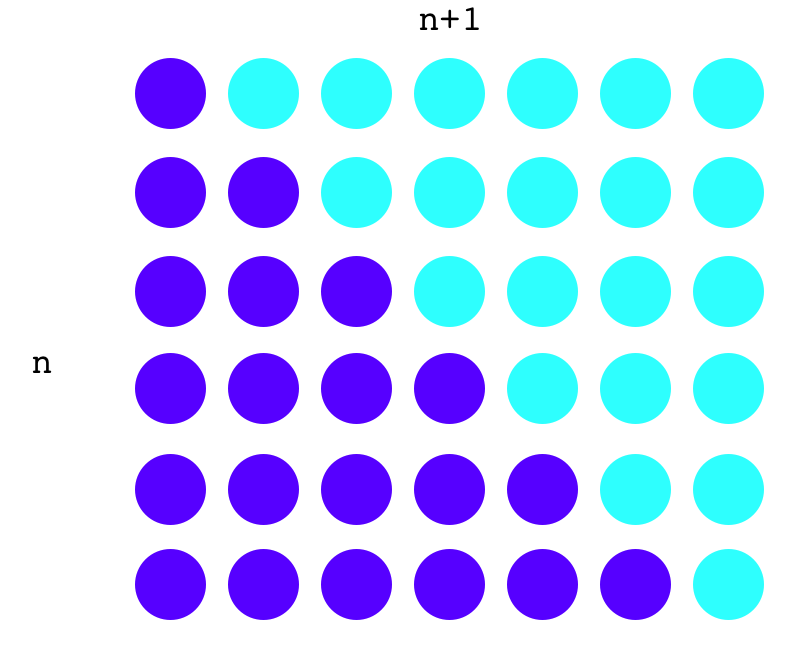
\includegraphics [scale=0.25] {sum_n.png}\end{center}
\[ 2S = n(n+1) \]
There is a famous story about Gauss that, as a schoolboy, he "saw" how to add the integers from $1$ to $100$ as two parallel sums
\[ \ \  1 + \ \ 2 + \ \ 3 + \cdots + 99 + 100 \]
\[ 100 + 99 + 98 + \cdots + 2 + 1 \]
Added together horizontally, these two series must equal twice the sum of $1$ to $100$.  But in the vertical, we notice that we have $n$ sums, each of which is equal to $n+1$.  So, again
\[ 2S = n (n+1) \]
\[ S = \frac{1}{2} \ n (n+1) \]
The value of the sum for $n=100$ is $5050$.  Another way of looking at this result is that between $1$ and $100$ there are $100$ representatives of the "average" value in the sequence, which (because of the monotonic steps) is $(100 + 1)/2 = 50.5$.  Or alternatively, view the sum as ranging from $0$ to $100$ (with the same answer).  Now there are $101$ examples of the average value ($100 + 0)/2 = 50$).

\subsection*{Digression on the method of induction}
\begin{center} 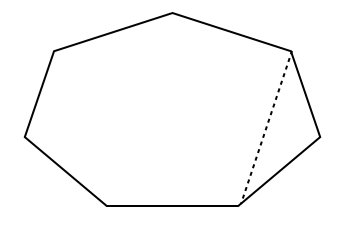
\includegraphics [scale=0.5] {polygon.png} \end{center}
I use my favorite example to introduce the method of induction.  In the figure above we have a polygon---an irregular heptagon.  Actually, there are two polygons, there is the heptagon with $n+1$ sides, and also the hexagon with only $n$ sides that would result from cutting along the dotted line.

What we would like to do is to find a formula for the sum of the internal angles that depends only on the number of sides or vertices.

The first part of the answer is to guess.  In the figure, you can see that by adding the extra vertex to go to the $n+1$-gon, we added a triangle, or perhaps you'd rather say than in going from $n+1$ to $n$ we lost a triangle.  In either case, the difference is $180^\circ$.  The difference between having $n$ sides and $n+1$ sides is to add $180^\circ$.  The second part of the argument is to suppose that $n=3$, in that case we must have simply $180^\circ$ degrees for a triangle.  So we guess that the formula may be
\[ (n-2)180^\circ = S_n \]
where S is the sum of the angles in an $n$-gon.
We can use induction to prove that this formula is correct.

Actually, we've already done the inducing part of induction, when we guessed the formula and verified it for one or a few cases.  Now we'd like to actually prove it.  The proof has two parts.  We must verify the formula for a base case like the triangle, which we've done.  You may wish to check that it works for the square as well, or even a line with two vertices, but that's not necessary.

The second part of the proof is to verify that in going from $n$ to $n+1$, we add another $180^\circ$.  \[ (n-2)180^\circ + 180^\circ \stackrel{?}{=} (n-1)180^\circ \]
On the left-hand side, we have the sum of angles for $n$ sides, which we assume is correct, and then we just add $180^\circ$ to it.  On the right, we have substituted $n+1$ into the formula $((n+1)-2=n-1)$.  Now we need to show that these are equivalent.
But of course
\[ (n-2)x + x = nx - 2x + x \]
\[ = nx + (-2 + 1)x \]
\[ = nx - x \]
\[ = (n-1) x \]
$\square$

That is the inductive proof of the formula.

We can visualize an inductive proof as a kind of chain.  We showed that the "base case" is true, for n = 3.  We also showed that if the formula works for n (when plugging into $n-2(180)=S$), it must work for n+1.

We know it works for $n = 3$;  therefore it works for $n = 4$

We know it works for $n = 4$;  therefore it works for $n = 5$

We know it works for $n = 5$;  therefore it works for $n = 6 \cdots$
\subsection*{Proof of the formula $n(n+1)/2$ by induction}

Returning to the sum of integers, one proof follows the method of induction.  In this approach, however, one must first guess the correct formula.  We guess $n(n+1)/2$, of course.  

Now, we \emph{assume} that the answer is correct for $n$.  We assume:
\[ S_n = \frac{n(n+1)}{2} \]
So clearly, if $S_n$ is correct, then
\[ S_{n+1} = S_n + (n + 1) \]
Follow out the arithmetic:
\[ = \frac{n(n+1)}{2} + \frac{2(n+1)}{2} \]
\[ = \frac{n(n+1) + 2(n+1)}{2} \]
\[ = \frac{(n+1)(n+2)}{2} \]

But this is precisely what we would obtain by using the formula, and substituting $n+1$ for $n$.  Hence the formula gives the correct result for $n+1$, assuming that it gives the correct result for $n$.  In turn, it gives the correct result for $n$, assuming it gives the correct result for $n-1$.  Eventually, we reach the base case, where we can actually verify that the result is correct.

Try it on the first value in the sequence (the "base case").
\[ \frac{1(1+1)}{2} = 1 \]
That checks.  So the whole chain of reasoning is correct.  $\checkmark$

\subsection*{Derivation using sums}
It seems a shame to spoil such a beautiful proof "without words" as the one above by saying anything more, but I can't resist.  I'd like to derive the equation we have been using using algebra.  The general method will help us later.

For any number, and in particular, any integer $k$ it is true that
\[ (k+1)^2 = k^2 + 2k + 1 \]
So consider what happens if we sum the values from $k=1 \rightarrow n$ for each of these terms
\[ \sum_{k=1}^n (k+1)^2 = \sum_{k=1}^n k^2 + \sum_{k=1}^n 2k + \sum_{k=1}^n 1 \]
If the sum is valid for any individual $k$, then it is also true plugging in all $k$ up to $n$.

Rearranging
\[ \sum_{k=1}^n (k+1)^2 - \sum_{k=1}^n k^2 = \sum_{k=1}^n 2k + \sum_{k=1}^n 1 \]
Now think about the left-hand side in our equation. 
\[ \sum_{k=1}^n (k+1)^2 - \sum_{k=1}^n k^2 \]
If we count down rather than up, start with $k=n$.  We have the following terms
\[ k = n \rightarrow \ \ (n+1)^2 - (n)^2 \]
\[ k = n-1 \rightarrow \ \ (n)^2 - (n-1)^2 \]
\[ k = n-2 \rightarrow \ \ (n-1)^2 - (n-2)^2 \]
\[ \cdots \]
\[ k = 1 \rightarrow \ \ (2)^2 - (1)^2 \]

Adding everything together, we obtain
\[ S = (n+1)^2 - (n)^2 + (n)^2 - (n-1)^2 + (n-1)^2 - (n-2)^2 + \cdots + (2)^2 - (1)^2 \]

Notice how all the terms except the first and last cancel.  This is called a "collapsing" or "telescoping" sum.  We have
\[ S = (n+1)^2 - 1 \]
\[ = n^2 + 2n \]

Bringing back the right-hand side  we have
\[ n^2 + 2n = \sum_{k=1}^n 2k + \sum_{k=1}^n 1 \]
We can bring the constant factor $2$ out of the sum, and also, we recognize that the sum of the value $1$ a total of $n$ times is just $n$.
\[ n^2 + 2n = 2\sum_{k=1}^n k + n \]

Subtract $n$ from both sides and divide by $2$:
\[ \sum_{k=1}^n k = \frac{n (n+1)}{2} \]
That's it!

\subsection*{Sum of Squares}
\begin{center} 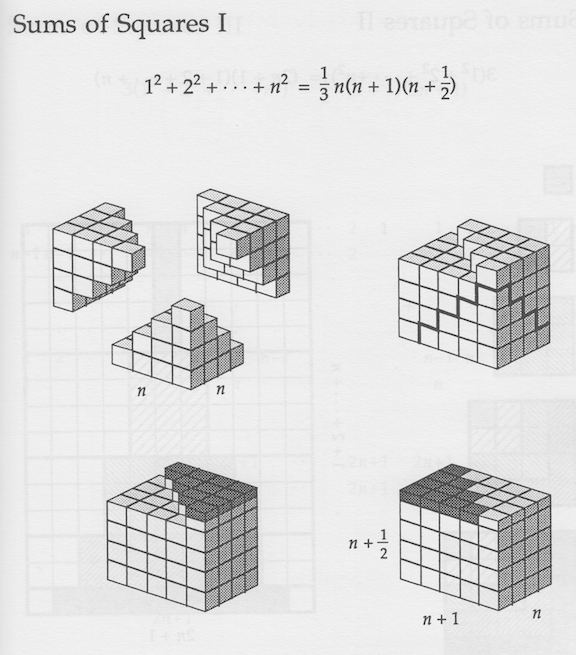
\includegraphics [scale=0.5] {sum_n2.png}\end{center}
Our next sum is that of the squares of the first $n$ integers.  There is a visual proof for this one as well (above).
\[ \sum_{k=1}^n k^2 \]
We obtain (by methods we will see below) the formula
\[ \sum_{k=1}^n k^2 = \frac{n(n+1)}{2} \cdot \frac{2n+1}{3} \]
\[ = \frac{n(n+1)(2n+1)}{6} \]
This formula is also written as
\[  \sum_{k=1}^n k^2 = \frac{1}{6} \ (2n^3 + 3n^2 + 2n) \]
\[ = \frac{n^3}{3} + \frac{n^2}{2} + \frac{n}{3} \]
We can check it by induction.  The base case is easy
\[ \frac{1(2)(3)}{6} = 1 \]  
$\checkmark$  

Now for the induction step:
\[ \frac{n(n+1)(2n+1)}{6} + (n+1)^2 \]
\[ = \frac{n+1}{6}  \ [ \ (n)(2n+1) + 6(n+1) \ ] \]
Look at what's in the brackets
\[ (n)(2n+1) + 6(n+1) \]
\[ = 2n^2 + 7n + 6 \]
\[ = (n + 2)(2n + 3) \]
\[ = (n + 1 + 1)(2(n + 1) + 1) \]
So altogether we have
\[ = \frac{(n+1)(n + 1 + 1)(2(n + 1) + 1)}{6} \]
which indeed, is the formula we had above, substituting $n+1$ for $n$.

\end{document}  